%%%%%%%%%%%%%%%%%%%%%%%%%%%%%%%%%%%%%%%%%%%%%%%%%%%%%%%%%%%%%%%%%
% Tese de Doutorado / Dept. Fisica, CFM, UFSC                   %
% Lacerda@Cidreira - Dez/2017                                   %
%%%%%%%%%%%%%%%%%%%%%%%%%%%%%%%%%%%%%%%%%%%%%%%%%%%%%%%%%%%%%%%%%

%:::::::::::::::::::::::::::::::::::::::::::::::::::::::::::::::%
%                                                               %
%                          Capítulo 1                           %
%                                                               %
%:::::::::::::::::::::::::::::::::::::::::::::::::::::::::::::::%

%***************************************************************%
%                                                               %
%                         Introdução                            %
%                                                               %
%***************************************************************%

\chapter{Introdução}
\label{sec:intro}

A forma empírica usual de estudarmos galáxias é através da luz emitida pelos seus constituintes. Mais precisamente, das imagens e da distribuição espectral de energia ({\em Spectral energy distribution}; SED\footnote{Quantidade de energia em cada comprimento de onda.}) que chegam até nossos telescópios, em terra ou no espaço. Diferentes componentes e eventos os modificam produzindo assinaturas características, nos possibilitando a busca de padrões e a criação de modelos que se propõem a explicar sua constituição, formação e dinâmica. Atualmente, existem diversos projetos astronômicos de levantamento de informações ou mapeamento de regiões do céu, chamados de {\em surveys}, formando uma rede de gigantescos bancos de dados de imagens, espectros e metainformação. Com diferentes faixas espectrais (desde raios-$\gamma$ até micro-ondas), diferentes fontes de dados (espectros de galáxias integradas, espectroscopia de campo, imagens, monitoramento temporal de eventos) e diferentes objetivos, os {\em surveys} astronômicos permeiam por diferentes fenônmenos astrofísicos. Através dessa criação e difusão em massa de informações, nossa forma de enxergar o mundo vem se tornando cada vez mais acurada quanto ao Universo. Além de estarem formando um imenso legado de informações para futuros astrofísicos, são basilares para o desenvolvimento de novas ideias e resolução dos desafios atuais da área. Neste capítulo faço uma introdução no assunto o qual esta tese está inserida, que se faz presente nesse cenário de `{\em art nouveau}' na astronomia, com um breve resumo dos avanços que nosso grupo de astrofísica (GAS-UFSC) tem obtido nos últimos anos.


%\section{Espectros integrados versus espectroscopia de campo}
\section{O todo e as partes}
\label{sec:intro:partes}

Galáxias são formadas por uma complexa mistura de gás, poeira, estrelas e matéria escura, distribuídas em discos, bojos e halos. Os primeiros grandes levantamentos de dados espectrais (\SDSS\footnote{\em Sloan Digital Sky Survey.}, \citealt{York.etal.2000a};
%COSMOS\footnote{\em Cosmic Evolution Survey},\citealt{Scoville.etal.2007};
2dFGRS\footnote{2dF Galaxy Redshift Survey.}, \citealt{Colless.etal.2001a}; são alguns exemplos) tratavam galáxias como uma fonte puntual de energia. Essa falta de informação espacial faz com que os padrões de diferentes partes com diferentes dinâmicas e regimes de ionização terminem misturadas no mesmo espectro, não sendo mais reconhecíveis. Apesar dessa limitação, muito se aprendeu (e ainda se aprende) sobre a formação e evolução das galáxias. Exemplos incluem a conexão entre o poder do núcleo ativo da galáxia ({\em active galactic nucleus}; AGN) e as populações estelares \citep{Kauffmann.etal.2003a}; a relação entre a taxa de formação estelar ({\em star-formation rate}; SFR) e a massa estelar das galáxias \citep{Brinchmann.etal.2004a}; a relação massa-metalicidade (MZR; \citealt{Tremonti.etal.2004a}); a evolução química e a história de formação estelar das galáxias \citep{CidFernandes.etal.2007, Asari.etal.2007a}; relação massa estelar-metalicidade \citep{ValeAsari.etal.2009a}; e mais importantes para o escopo desta tese, a revelação de uma imensa e esquecida população de galáxias aposentadas ionizadas por estrelas quentes de baixa massa em alto estado de evolução ({\em hot low-mass evolved stars}; HOLMES) \citep{Stasinska.etal.2008a, CidFernandes.etal.2010a, CidFernandes.etal.2011a}.

Quando apenas um espectro representa uma galáxia podemos perceber que qualquer propriedade que varie em função da posição será erroneamente estimada. Outro problema acontece quando estimamos propriedades referentes a diferentes regimes de ionização na galáxia, como a metalicidade nebular\footnote{Quantidade de elementos diferentes de Hidrogênio e Hélio presentes no gás que está formando estrelas, estimada geralmente utilizando a razão entre a abundância do Oxigênio e a do Hidrogênio.} por exemplo. Nesse caso, devemos levar em conta apenas os fótons gerados nas regiões de formação estelar ({\em star-forming}; SF), isolando-os daqueles que vêm de outros regimes nebulares, como o gás difuso ionizado ({\em diffuse ionized gas}; DIG), fotoionização pelo núcleo ativo ou estrelas velhas. Dessa forma, para um estudo mais preciso das propriedades derivadas dos espectros integrados e, por consequência, do viés causado por construção dos espectros, um melhor entendimendo desses efeitos se faz necessário.

Um grande passo nessa direção foi dado com a criação dos {\em surveys} de espectroscopia de campo integral ({\em integral field spectroscopy}; IFS). Através da IFS podemos desvencilhar essa mistura de partes distintas, pois nessa técnica de observação temos espectros para cada parte da galáxia. Assim, para cada par espacial ($x,y$) temos uma dimensão espectral $\lambda$. Quanto maior o intervalo de comprimento de onda e melhores as resoluções espacial e espectral teremos uma mais completa definição da localização e da natureza espectral de cada uma das partes do objeto observado. Diversos {\em surveys} IFS já estão finalizados e com seus dados disponíveis publicamente (CALIFA\footnote{\em Calar Alto Legacy Integral Field Area survey.} DR3\footnote{\em Data-release 3.}, \citealt{SFSanchez.DR3.2016}; PINGs\footnote{\em PPAK IFS Nearby Galaxies survey.}, \citealt{RosalesOrtega.etal.2010}), outros ainda estão em fase de observação e com alguns dados já disponíveis (MaNGA\footnote{\em Mapping nearby Galaxies at Apache Point Observatory.} \SDSS-IV DR13, \citealt{MaNGADR1.2017}; SAMI\footnote{equipamento e {\em survey} são homônimos; {\em Sydney-AAO Multi-object Integral-field spectrograph.}} DR1, \citealt{SAMIDR1.2017}). Com o desenvolvimento de novos equipamentos como o MUSE\footnote{{\em The Multi Unit Spectroscopic Explorer} - \href{https://www.eso.org/sci/facilities/develop/instruments/muse.html}{https://www.eso.org/sci/facilities/develop/instruments/muse.html}} e o SITELLE\footnote{{\em Spectromètre Imageur à Transformée de Fourier pour l'Etude en Long et en Large de raies d'Emission}; \href{http://cfht.hawaii.edu/Instruments/Sitelle/}{http://cfht.hawaii.edu/Instruments/Sitelle/}} poderemos estudar galáxias e suas interações com ainda mais detalhes.

Nessa direção, este trabalho utiliza dados de IFS do CALIFA para estudar a importância e a caracterização do DIG em diferentes regiões de galáxias cobrindo todos os tipos de Hubble\footnote{Edwin Hubble criou o diagrama de morfologia de galáxias, conhecido hoje como classificação de Hubble, classificando-as como elípticas, espirais, e irregulares. As galáxias de elipticas são conhecidas como de tipo precoce ({\em early-type galaxies}) e as espirais são conhecidas como de tipo tardio ({\em late-type galaxies}).}. A completa cobertura de galáxias com diferentes morfologias e diferentes inclinações faz do CALIFA um {\em survey} ideial para esse tipo de estudo, mesmo sabendo que a resolução espacial não nos permite uma descrição detalhada das diferentes componentes do meio interestelar ({\em interstellar medium}; ISM). Estudos utilizando IFS com melhor resolução já existem \citep{Sanchez.etal.2015MUSE, Vogt.etal.2017a, RousseauNepton.etal.2017}, mas como cobrem tão poucos objetos não podemos usá-los para um estudo mais geral como esse.


\section{O GAS-UFSC e o IAA-CSIC}
\label{sec:intro:UFSCeIAA}

Nos últimos anos nosso grupo de Astrofísica (GAS-UFSC) aqui na Universidade Federal de Santa Catarina vem trabalhando com dados de diversos {\em surveys}. Nosso grupo foi pioneiro no estudo das propriedades físicas das populações estelares de aproximadamente um milhão de galáxias do \SDSS através do projeto SEAGal/\starlight\footnote{\href{http://starlight.ufsc.br}{http://starlight.ufsc.br}} publicando diversos artigos importantes e amplamente citados \citep[e.g., ][]{CidFernandes.etal.2005a, Mateus.etal.2006a, Stasinska.etal.2006a, Asari.etal.2007a, Stasinska.etal.2008a, CidFernandes.etal.2011a}.

Durante esse trabalho, nosso grupo de estudo de populações estelares seguiu participando de um projeto com pesquisadores do Instituto de Astrofísica de Andalucía (IAA), na cidade de Granada, Comunidade autônoma de Andalucía, ao sul da Espanha. Esse instituto pertence ao {\em Consejo Superior de Investigaciones Científicas} (CSIC), o maior órgão público (estatal) de pesquisas científicas na Espanha, e o terceiro maior da Europa. Conta com pesquisadores participantes do \CALS, funcionando como centro físico do projeto. A pesquisadora Rosa M. González Delgado, coorientadora deste trabalho, uma das principais líderes do projeto e que também atuou como Pesquisadora Visitante Especial (PVE-CsF) aqui na UFSC; Rubén García Benito, que faz parte do grupo de redução dos dados do {\em survey}; e Enrique Pérez, do grupo de populações estelares; já trabalham em nossa parceria e possuem conhecimento e domínio das técnicas exploradas por nosso projeto, além de participarem ativamente do desenvolvimento do CALIFA. Durante os últimos cinco anos nosso grupo de populações estelares no CALIFA publicou diversos artigos e quatro teses de doutorado. Paralelamente participamos de diversos congressos e conferências publicando nossos resultados. Detalhes técnicos e comparações entre {\em surveys} IFS podem ser encontrados em \citet{Andre2015}.

\subsection{\starlight + CALIFA}
\label{sec:intro:UFSCeIAA:SLCAL}
Um dos maiores frutos de toda essa parceria é nossa participação no projeto CALIFA. Dentro dele, nós analisamos todos os cubos de dados dos objetos observados utilizando o código de síntese espectral \starlight e a plataforma PyCASSO ({\em Python CALIFA \starlight synthesis organiser}), descritos em \citet{CidFernandes.etal.2013a, CidFernandes.etal.2014a} e em \citet{deAmorim.etal.2017}. Com a síntese de populações estelares pode-se modelar os espectros proveniente das estrelas de diferentes idades e composições químicas (metalicidade), além da correção pela aplicação de uma lei de extinção por poeira. Essa análise foi basilar para a série de estudos que aconteceram nos últimos anos, resolvendo as populações estelares destes objetos no espaço e no tempo pela primeira vez. Aqui um rápido resumo do que nós desenvolvemos até agora:

\begin{enumerate}[label=(\roman*)]
  \item Através da história de formação estelar ({\em star-formation history}; SFH) espacialmente resolvida, em \citet{Perez.etal.2013a} pudemos, pela primeira vez, traçar a história do crescimento da massa estelar de $\sim 100$ galáxias em função da distância radial. O resultado, que sugere que galáxias crescem de dentro para fora, foi confirmado por \citet{RGB.etal.2017} com uma amostra sete vezes maior.
  \item Informações espacialmente resolvidas e mapas 2-D das populações estelares foram usados para recuperar relações locais entre:
  \begin{enumerate*}[label=(\alph*)]
    \item densidade superficial de massa estelar, $\Sigma_\star$, e idades estelares médias ponderadas pela luz, \meanL{\log t} \citep{GonzalezDelgado.etal.2014a};
    \item metalicidade estelar média ponderada pela massa, \meanM{\log Z}, e $\Sigma_\star$ \citep{GonzalezDelgado.etal.2014b};
    \item a densidade superficial da taxa de formação estelar, $\Sigma_{\rm SFR}}$, que funciona como um sensor de intensidade de formação estelar, e $\Sigma_\star$ \citep{GonzalezDelgado.etal.2016a}.
  \end{enumerate*}
  Estes estudos serviram para mostrar que os processos locais empregam papel fundamental regulando a formação estelar e enriquecimento químico no disco de galáxias espirais. Já nos esferóides esses processos são regulados pela massa estelar total, $M_\star$. Além do mais, com a comparação entre análise espectral integrada e espacialmente resolvida, encontramos que as propriedades das populações estelares são bem representadas por seus valores a 1 HLR\footnote{Half-light radius. Raio que contém metade da luz da galáxia na janela espectral de normalização dos espectros.} \citet{GonzalezDelgado.etal.2014a}.
  \item Estudando os perfis radiais de diversas propriedades físicas como a extinção estelar, $A_V$, $\Sigma_\star$, \meanL{\log t}, \meanM{\log Z} e seus gradientes em função da distância radial confirmamos que galáxias mais massivas são mais compactas, velhas, evoluídas quimicamente e menos avermelhadas por poeira. A dispersão nesses perfis parecem correlacionar com o tipo morfológico mostrando que para uma mesma $M_\star$, as galáxias mais {\em early-types} são também mais compactas, velhas e mais evoluídas quimicamente, o que evidencia que a cessão de formação estelar está relacionada ao tipo morfológico \citep{GonzalezDelgado.etal.2015a}. Nesse mesmo artigo vimos que os gradientes negativos de \meanL{\log t} e \meanM{\log Z} confirmam que galáxias crescem de dentro para fora.
  \item As estruturas radiais de $\Sigma_{\rm SFR}$ e a dispersão muito pequena desses perfis radiais entre galáxias espirais nos confirmaram que a sequência principal de galáxias formadoras de estrelas ({\em main sequence of star-formation galaxies}; MSSF) é praticamente constante em $\Sigma_{\rm SFR}$. Os gradientes positivos dos perfis da taxa de formação estelar específica local e recente (sSFR) e o seu aumento ao irmos das galáxias {\em early-} para as {\em late-types} também sugerem que galáxias param a formação estelar de dentro para fora e esse processo acontece mais rápido em galáxias dominadas pelo bojo e não pelo disco \citep{GonzalezDelgado.etal.2016a}. Nesse mesmo estudo, graças a função de seleção bem definida do CALIFA \citep{Walcher.etal.2014} pudemos estimar a densidade de SFR no Universo local em $0.0105 \pm 0.0008\,$M$_\odot\,$yr$^{-1}\,$Mpc$^{-3}$, de acordo com outros estudos independentes.
  \item Com os mapas 2-D da evolução temporal e espacial da SFH das galáxias pudemos estimar a evolução temporal da SFR, sua intensidade ($\Sigma_{\rm SFR}$) e a sSFR. Nós encontramos que galáxias se formam muito rápido independentemente de sua massa estelar, resultando em um pico de formação estelar em alto {\em redshift} ($z \sim 2$), e que a formação estelar subsequente é guiada por $M_\star$ e pela morfologia, com os tipos espirais mais tardios formando estrelas por um periodo mais longo de tempo \citep{GonzalezDelgado.etal.2017}.
  \item Estudos de objetos em interação ({\em mergers}) e suas comparações com galáxias espirais `não-interagentes' nos revelam o papel que a interação tem sobre as história de formação estelar, qual sua extensão de atividade e também uma estimativa da época do início da interação \citep{CortijoFerrero.etal.2017a, CortijoFerrero.etal.2017b, CortijoFerrero.etal.2017c}.
  \item Atualização do \starlight que nos possibilitou a análise das populações estelares de uma forma mais precisa unindo dados fotométricos no ultra-violeta (UV) do GALEX\footnote{\em Galaxy Evolution Explorer survey.} \citep{Martin.etal.2005} com os espectros ópticos do CALIFA \citep{LopezFernandez.etal.2016}. Dessa forma, há uma significante diminuição nas incertezas nas propriedades estelares. Também obtemos uma melhora na resolução das populações mais jovens, pois elas contribuem majoritariamente no UV.
  \item Publicação de um banco de dados\footnote{\href{http://pycasso.ufsc.br}{http://pycasso.ufsc.br} ou \href{http://pycasso.iaa.es}{http://pycasso.iaa.es}} com todos os resultados da síntese de populações estelares utilizando o \starlight para 445 galáxias do DR3 do CALIFA \citep{deAmorim.etal.2017}.
\end{enumerate}

Todos esses resultados provém da análise das populações estelares, mas com a síntese podemos ir além. Através dos espectros residuais podemos estudar as linhas de emissão que nos servem de fonte para estimar propriedades do gás \citep{Asari.etal.2007a}, como veremos na próxima seção.

\subsection{Linhas de emissão}
\label{sec:intro:UFSCeIAA:EmLines}
Espectros observados carregam uma mistura de luz provenientes das distintas componentes das galáxias (estrelas, gás, poeira, etc). Subtraindo os espectros observados dos espectros modelados pela síntese obtemos os espectros residuais, compostos basicamente pelas linhas de emissão. Essas linhas são geradas principalmente através das ionizações e recombinações de átomos dos elementos encontrados no meio interestelar, e mais densamente, nas nuvens de gás.

Dentre os diversos produtos indiretos da síntese de populações estelares, a medida dos fluxos integrados das linhas de emissão é peça fundamental em nosso projeto. Esse processo foi feito utilizando o {\sc sherpa} IFU line fitting software \citep[SHIFU;][]{RGB.etal.2017}, baseado no pacote {\sc ciao's sherpa} \citep{Freeman.etal.2001, Doe.etal.2007}. Esse programa ajusta perfis gaussianos nas linhas de emissão presentes nos espectros residuais, além de estimar os erros envolvidos neste processo. Um exemplo pode ser observado na Fig.\ \ref{fig:rgbline}. Nela vemos a linha de \Hb na zona central do objeto UGC00148 e o ajuste feito pelo programa.

\begin{figure}
	\centering
	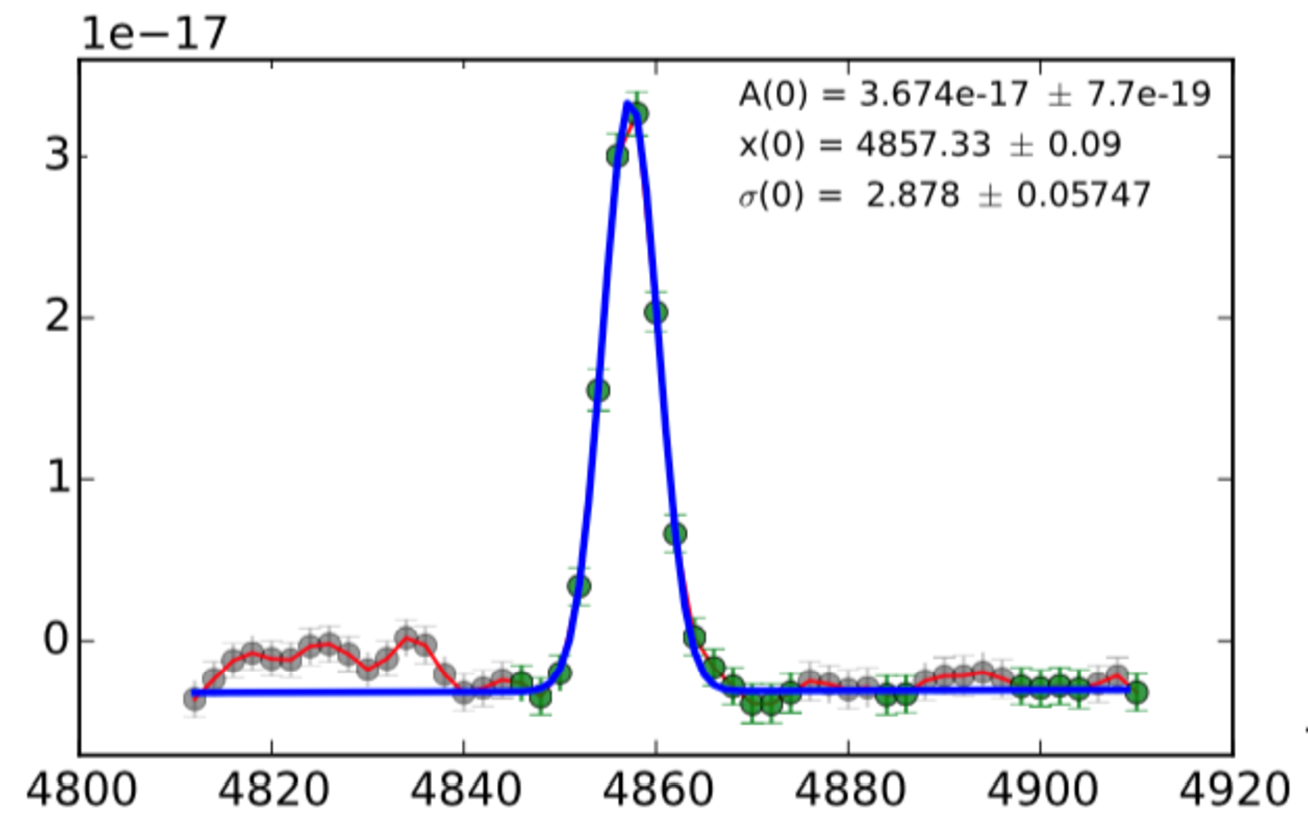
\includegraphics[scale=0.4]{figuras/K0012-zone0-Hb.pdf}
	\caption[Exemplo de ajuste de linha de emissão]
	{Espectro na região da linha de \Hbeta em emissão para a zona central da galáxia UGC00148 (objeto
CALIFA 12) juntamente com o melhor ajuste utilizando uma gaussiana. Em destaque a amplitude (A), o
comprimento de onda central (x) e o desvio padrão neste ajuste (\sigma).}
	\label{fig:rgbline}
\end{figure}


\section{Gás ionizado difuso (DIG)}
\label{sec:intro:DIG}

\subsection{Primeiras detecções}
\label{sec:intro:DIG:first}
O DIG foi detectado pela primeira vez no disco Galáctico através de linhas de emissão fracas fora de regiões \Hii\footnote{Regiões formadoras de estrelas; são formadas por imensas nuvens de gás molecular, originado pelo esfriamento de gás do meio interestelar, que se fragmentam formando estruturas menores e cada vez mais densas.} clássicas \citep{Reynolds.PhD.1971}. Observações de galáxias espirais {\em edge-on} através de imageamento em \Ha \citep{Dettmar.1990, HoopesWaltGreen.1996, HoopesWaltRand.1999} mostraram a existência de DIG a grandes distâncias do plano galáctico. \cite{Oey.etal.2007}, estudando 109 galáxias do SINGS\footnote{\em Spitzer Infrared Nearby Galaxies Survey.}, chegaram à conclusão que emissão difusa em \Ha está presente em galáxias de todos os tipos de Hubble e representa $\sim60\%$ da emissão total em \Ha, independentemente do tipo morfológico ou da SFR total.

\subsection{Fonte de ionização do DIG}
\label{sec:intro:DIG:source}
Fótons de estrelas massivas do tipo OB escapando das regiões \Hii é a fonte de ionização mais comumente adotada para explicar as linhas de emissão no DIG (veja o review em \citealt{Haffner.etal.2009}). Entretanto, razões de linhas como \nii/\Ha, \sii/\Ha, and \oiii/\Hb crescem com a altura em relação ao plano galáctico, fazendo com que seja necessário a inclusão de fontes adicionais (ou alternativas) de ionização. \citet{HoopesWalt.2003} estudaram essas razões de linhas em regiões de DIG em algumas galáxias e chegam a conclusão que nem ionização por estrelas quentes e massivas e nem fótons que escaparam de regiões \hii podem explicar por si a ionização do DIG.

Diversas são as fontes que poderiam gerar esse adicional de ionização. As mais citadas são choques \citep{CollinsRand.2001}, mistura turbulenta de camadas do meio interestelar \citep{SlavinShullBegelman.1993, Binette.etal.2009a}, reconexão magnética, raios cósmicos ou emissão fotoelétrica proveniente de pequenos grãos \citep{Reynolds.etal.2001} e HOLMES \citep{FloresFajardo.etal.2011a}. Em \citet{Stasinska.etal.2008a} e em \citet{CidFernandes.etal.2011a} HOLMES também foi invocado como fonte de ionização de galáxias aposentadas que apresentam linhas de emissão muito fracas. Esses sistemas pararam de formar estrelas há muito tempo e são ionizados por suas populações de estrelas velhas e quentes, produzindo razões de linhas de emissão do mesmo tipo daquelas em regiões nucleares de baixa ionização ({\em low-ionization nuclear emission-line region}; LINER), um fenômeno que é comum em galáxias elípticas e em bojos de galáxias espirais \citep{Sarzi.etal.2010, Gomes.etal.2016a, Belfiore.etal.2016}.

Independentemente da fonte que alimenta o DIG, seu regime nebular é diferente daquele das regiões \hii, com densidades menores, menor parâmetro de ionização e temperaturas eletrônicas mais altas, portanto, não podemos negligenciar sua existência quando estamos derivando propriedades de galáxias.

\subsection{Como separar regiões DIG e SF}
\label{sec:intro:DIG:class}
As regiões de DIG e SF são separadas geralmente utilizando como base o brilho superficial de \Ha ($\Sigma_{\Ha}$) por sua relação direta com a densidade do gás ionizado. \citet{Zhang.etal.2017a}, por exemplo, usa $\Sigma_{\Ha} > 10^{39}$ erg$\,$s$^{-1}\,$kpc$^{-2}$ como critério para selecionar {\em spaxels} ({\em spectral pixels}) confiantemente dominados por regiões \hii. Outros estudos não utilizam apenas um valor limite, mas ainda sim embasados em $\Sigma_{\Ha}$ (veja a discussão em \citealt{Zurita.etal.2000}, \citealt{Oey.etal.2007} e \citealt{Vogt.etal.2017a}). No entanto, esse {\em approuch} não é totalmente adequado, como veremos no Capítulo \ref{sec:DIGclass}. A separação utilizando como base $\Sigma_{\Ha}$ é conceitualmente incorreta, podendo levar a inconsistências nos resultados sob certas circunstâncias. Além do mais, $\Sigma_{\Ha}$ não nos dá pista alguma sobre a natureza da emissão no DIG.

A fim de solucionar esse problema levamos em conta o papel do contínuo espectral utilizando a largura equivalente de \Ha, $W_{\Ha}$, em nosso sistema de classificação. Como mostramos no artigo \citet[][Apêndice \ref{apendice:DIGpaper0}]{Lacerda.etal.2018}, linha principal desta tese, $W_{\Ha}$ consegue com sucesso diferenciar qualitativamente regimes SF e DIG. Seguindo a linha traçada por \citet{Binette.etal.1994a}, \citet{Stasinska.etal.2008a} e \citet{CidFernandes.etal.2011a} na identificação de HOLMES como fonte de ionização de galáxias elípticas e de \citet{FloresFajardo.etal.2011a} identificando esses como a provável fonte de ionização do DIG extra-planar, somos capazes de identificar elegantemente o gás presente no DIG que é ionizado por HOLMES, o hDIG. As regiões remasnescentes (nem ionizadas apenas por HOLMES nem por SF) são provavelmente uma mistura de processos, e serão classificadas como DIG misto, o mDIG ({\em mixed} DIG).

Regiões \Hii possuem alguns {\em parsecs} de extensão, com algumas chegando até 0.1--0.3kpc (gigantes regiões como 30 Doradus ou NGC 604; e.g. \citealt{Rosa.y.Enrique.2000}). A resolução espacial do CALIFA de $\sim 0.8kpc$ excede esse limite, portanto, nossas regiões classificadas como SF, por construção, contém alguma emissão difusa. Essa característica é ainda mais evidente nas regiões onde existam algum tipo de binagem espacial e, por esse motivo, daqui em diante usaremos o termo SFc ({\em star-forming complexes}\footnote{Complexos de formação estelar.}) como denominzação dessas regiões em que a razão entre SF/DIG é grande.


\section{Este trabalho}
\label{sec:intro:estetrabalho}

Essa tese é um apanhado de alguns dos trabalhos no qual participei durante o tempo do doutorado, com foco principal no artigo sobre a natureza das linhas de emissão das regiões das galáxias do CALIFA, separando aquelas SF daquelas melhores caracterizadas como DIG. No Cap.\ \ref{sec:sample} apresento a amostra de galáxias utilizadas neste trabalho. O artigo principal será dividido em dois capítulos. A apresentação do método de caracterização está no Cap.\  \ref{sec:DIGclass}, e no próximo (Cap.\ \ref{sec:DIGdisc}) fazemos a discussão sobre esse método de classificação de regiões e a análise das regiões classificadas. Por fim, demais artigos e trabalhos são apresentados no Cap.\ \ref{sec:more}.

% \subsection{Artigo - CALIFA, the Calar Alto Legacy Field Area survey IV. Third public data release.}
% \label{sec:intro:UFSCeIAA:DR3}
%
% Houveram três lançamentos públicos dos dados armazenados pelo CALIFA durante o decorrer do projeto, finalizando com o DR3\footnote{\em Data-release 3} (\citealt{SFSanchez.DR3.2016}, que também pode ser encontrado no Apêndice \ref{apendice:SFSanchezDR3} deste trabalho). Este DR conta com espectros de 667 galáxias ($\sim 1,5$ milhões de espectros) com tipos morfológicos cobrindo toda a classificação de Hubble e redshifts variando entre 0.005 e 0.03 (distâncias de 20 a 130 Mpc).
%
% Nosso grupo de populações estelares se encarregou de escrever alguns programas de análise e gerar as imagens nas quais nos embasamos para avaliar a qualidade da síntese de populações estelares com o \starlight para distintas posições em cada galáxia, além de realizarmos uma comparação com os resultados para a amostra do DR1 \citep{Husemann.etal.2013a}.  e do DR2 \citealt{GarciaBenito.etal.2015a}. Durante esse trabalho notamos que os resíduos reduziram sensivelmente desde a última versão. Esta mesma análise nos ajudou a melhorar a máscara de remoção de linhas telúricas\footnote{Linhas provenientes de fenômenos que ocorrem na Terra.} dos espectros. Também verificamos que os erros relacionados aos espectros observados possuem uma distribuição muito próxima a uma gaussiana.
